\documentclass[a4paper]{report}
    
    \usepackage{D:/cours/INGESUP/package/model}    
    
    \title{Statistiques}
    \author{
        Antoine Lucsko \\
        {\small \href{mailto: antoine.lucsko@gmail.com}{antoine.lucsko@gmail.com} }
    }
    \date{2017-09-01}
    
    \begin{document}
        \selectlanguage{francais}	
        \tableofcontents
        \maketitle
        
        \begin{abstract}
            Objectifs: Statistiques
        \end{abstract}
    
    \chapter{Introduction}
    Le but des statistiques est d'induire des lois de comportement à partir d'un grand nombre d'observations ou de données. En particulier, on cherchera la corrélation entre deux caractères X et Y partagés par les individus d'une population. \\
    \begin{figure}[!h]
        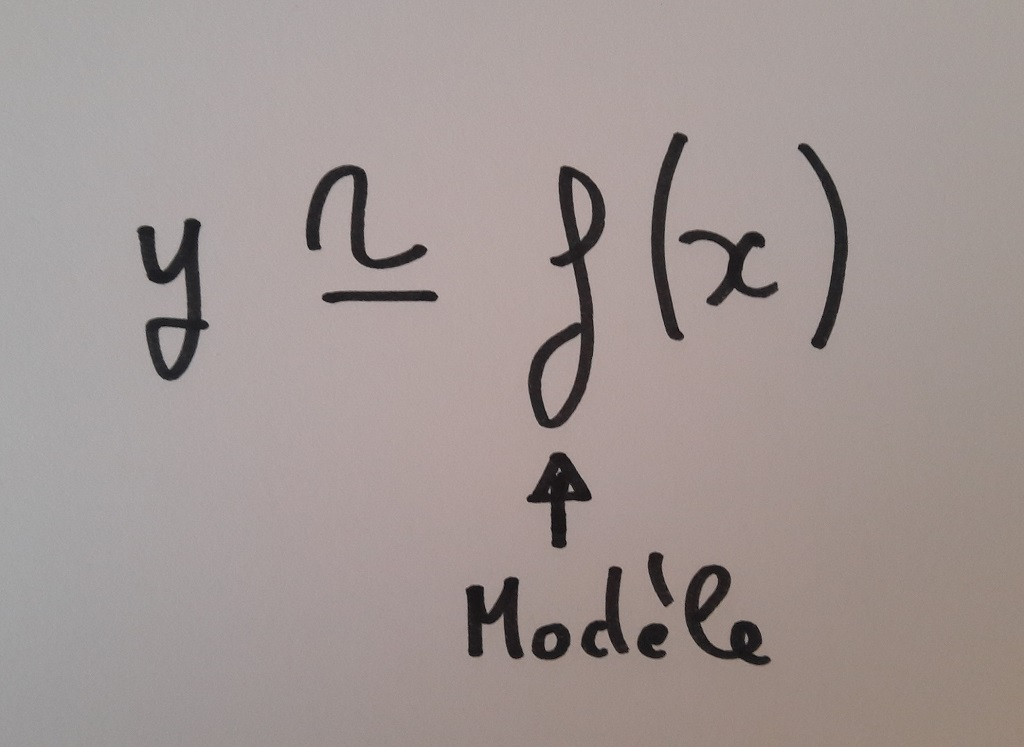
\includegraphics[width=8cm]{../Images/stat01}
    \end{figure}

    \pagebreak

    \chapter{Nuages de points}
    \section{Définition série double}
    On définit une série statistique double $(x,y) =((x_1, ..., x_n),(y_1, ..., y_n)) $ en observant deux caractères ou variables sur une même population de taille n. L'ensemble des points de coordonnées $(x_i,y_i)$, rapportés dans un repère du plan, forme le nuage de points de la série (x,y).
    \section{Définition Point moyen}
    Le point G de (x,y) est le point dont les coordonnées sont les moyennes des séries: \\
    $x_G = \frac{1}{n}(x_1+...+x_n)$ \\
    $y_G = \frac{1}{n}(y_1+...+y_n)$ \\
    \begin{figure}[!h]
        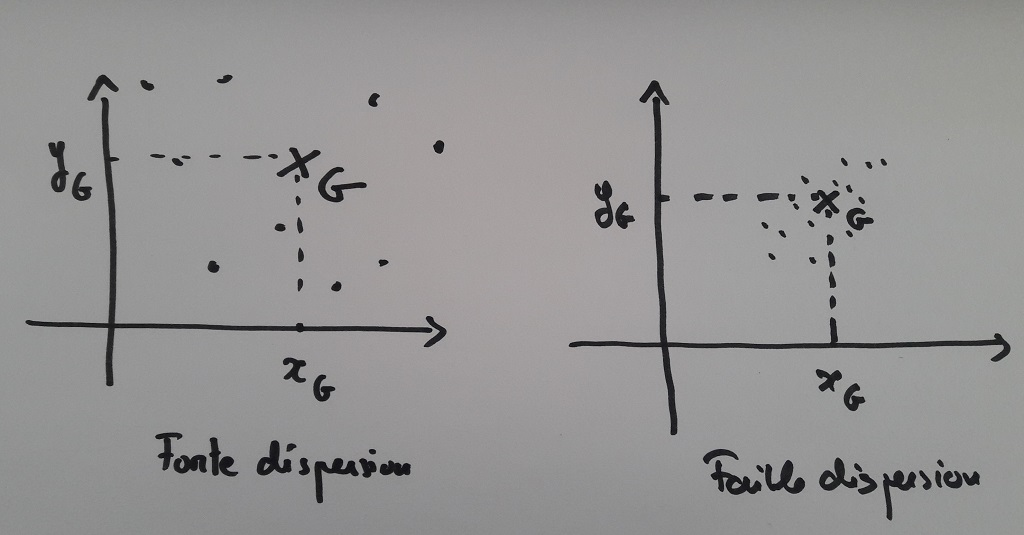
\includegraphics[width=8cm]{../Images/stat02}
    \end{figure}

    \pagebreak
    \section{Covariance et écart type}
    La variance et l'écart type sont deux indicateurs de dispersion des valeurs d'une série x autour. La Covariance mesure la tendance qu'ont les deux variables à varier ensemble,\textbf{c'est-à-dire à être dépendantes l'une de l'autre}. Par exemple si une des deux variables varie beaucoup tandis que l'autre varie peu alors la covariance est faible. \\
    Une covariance négative signifie que l'une des deux variables croit tandis que l'autre décroit et une variance positive réciproquement. \\
    \\
    $cov(x,y) = \sigma(x,y) = \frac{1}{n} \sum_{i=1}^n(x_i-\bar{x})(y_i-\bar{y})$
    \\ \\
    $cov(x,y) = \sigma(x,y) = \frac{1}{n} (\sum_{i=1}^nx_i \times y_i) - \bar{x} \times \bar{y}$
    \pagebreak
    \section{Ajustement affine par moindre carrés}
    Si les points du nuage paraissent presque alignés on peut décider d'un ajustement affine, c'est-à-dire de modéliser le nuage par une droite. \textbf{Il faut donc trouver une droite au plus prêt des points du nuage}.
    \begin{figure}[!h]
        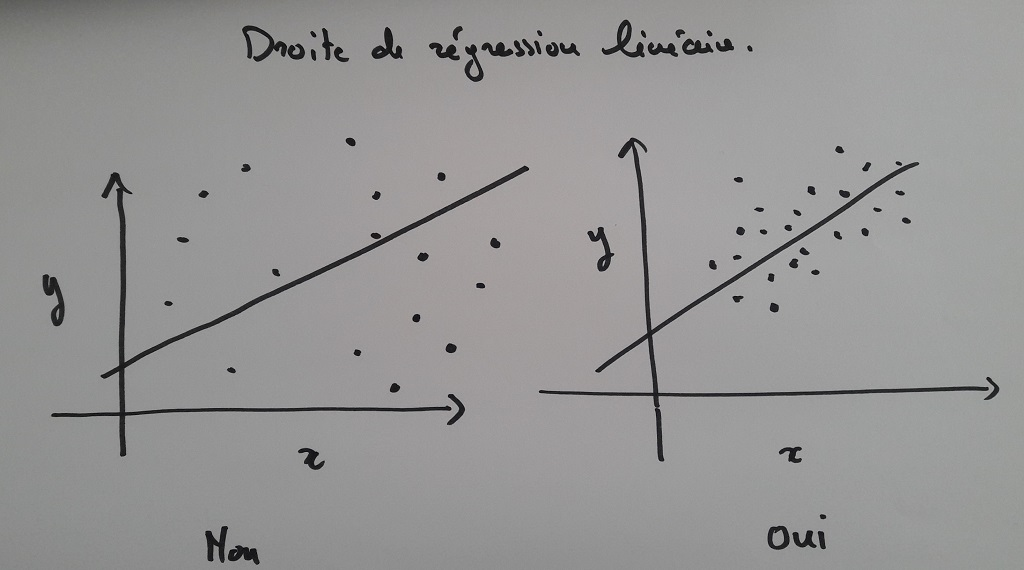
\includegraphics[width=8cm]{../Images/stat03}
    \end{figure} \\
    Voici l'erreur quadratique totale entre la droite et le nuage de points: \\ \\
    $\sum_{i=1}^n(y_i - (ax_i+b))^2$
    \\ \\
    Voici l'équation de la droite de régression :\\
    $y -\bar{y} = \frac{\sigma(x,y)}{\sigma(x)} (x-\bar{x}) $, remarquez que la droite passe par le point moyenne G.
    
    \pagebreak
    \section{indicateur de corrélation}
    Le coefficient de corrélation entre deux variables aléatoires réelles X et Y ayant chacune une variance finie est noté $\rho(X,Y) = \frac{Cov(X,Y)}{\sigma(X) \times \sigma(Y)}$. \\
    Si ce dernier est égale à 1 alors y est une fonction affine de x ou réciproquement. \\
    Si ce coefficient est proche de 1 ou -1 les deux variables X et Y sont d'autant mieux corrélées. \\
    Si ce coefficient est nul cela signifie que les deux variables ne sont pas corrélées linéairement.
    \begin{figure}[!h]
        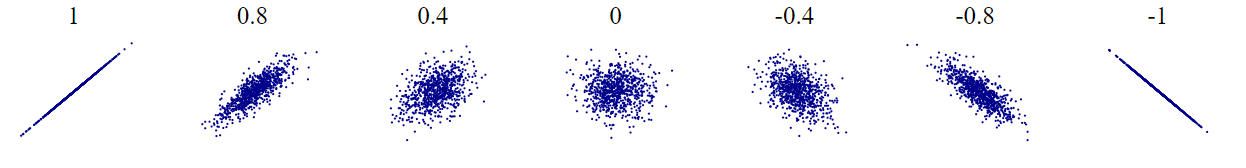
\includegraphics[width=8cm]{../Images/stat06}
    \end{figure}
    \pagebreak
    \section{Croissance exponentielle}
    Lorsque l'on place de l'argent sur un compte en banque, alors l'argent croît exponentiellement et non linéairement: \\ \\
    Techniquement, on obtient un ajustement exponentiel en effectuant au préable un changement de variable sur la série y en posant $z = \ln{y}, z = ax + b$, $y=\exp{(ax+b)}$ \\
    \begin{figure}[!h]
        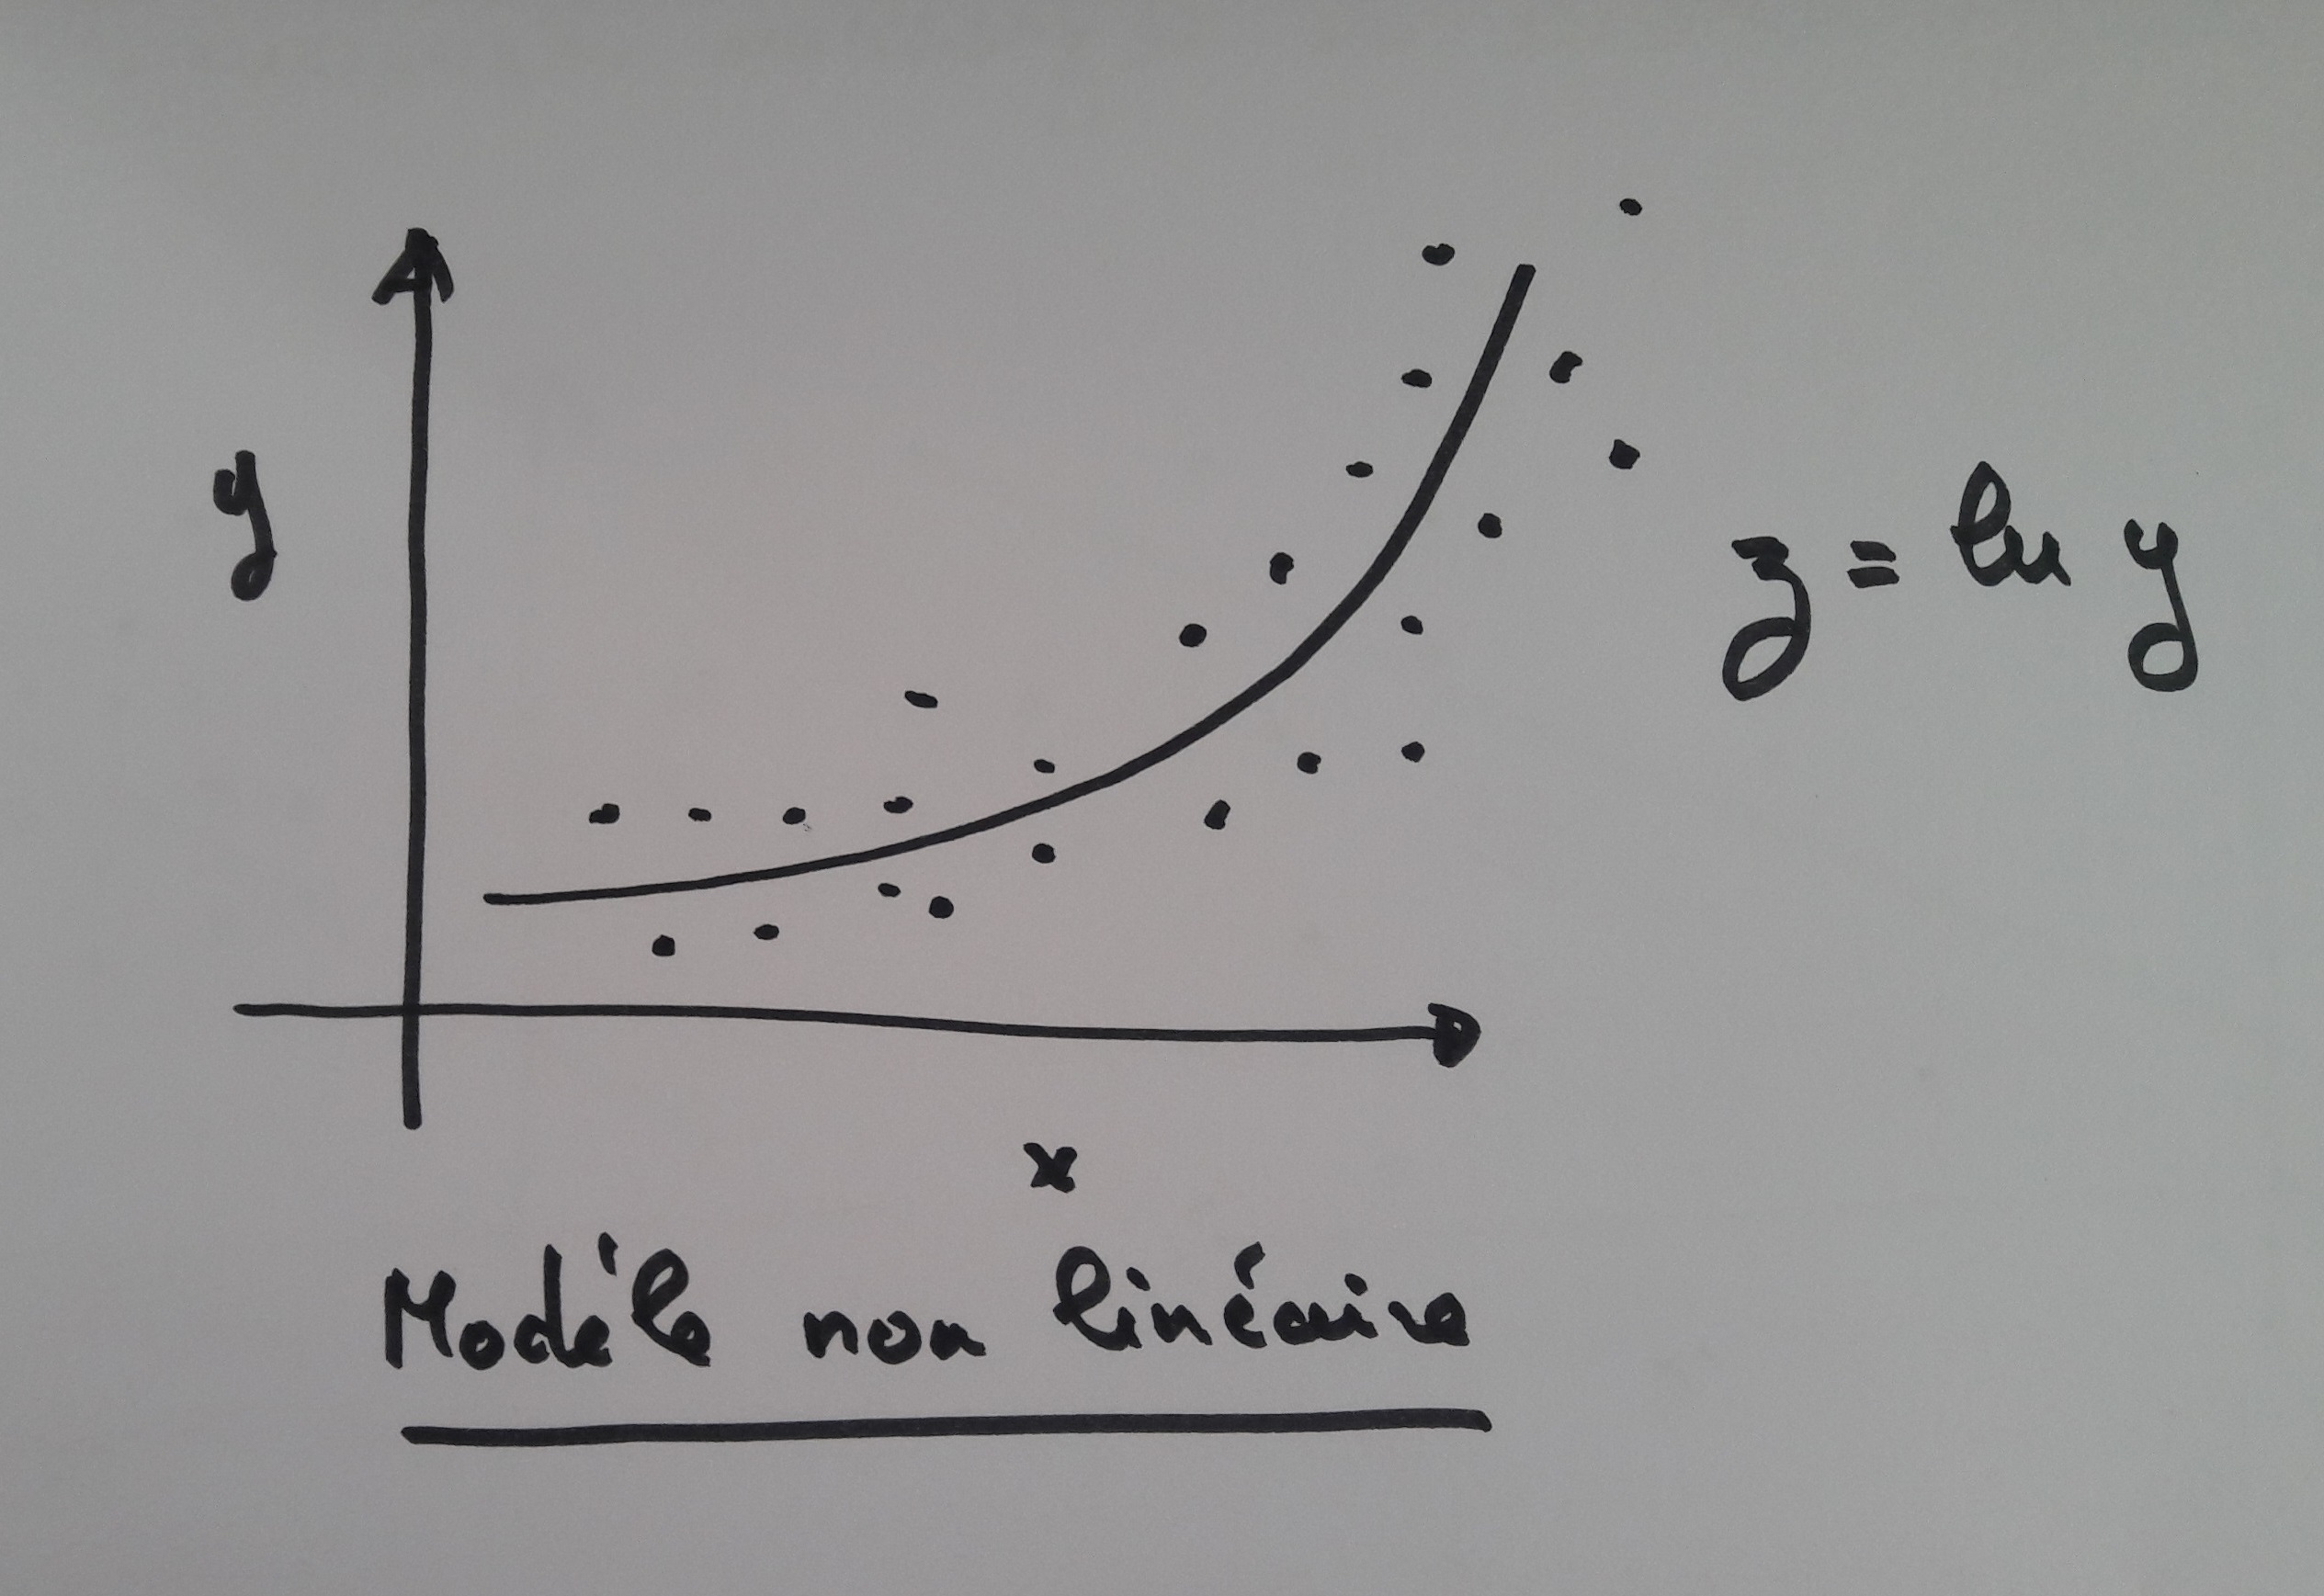
\includegraphics[width=8cm]{../Images/stat04}
    \end{figure} \\

    \pagebreak
    \section{Moyennes géométrique}
    On connait la moyenne arithmétique classique. Supposons maintenant que nous aillons à calculer les intérêts que rapporte une somme placée sur deux ans.
    \begin{figure}[!h]
        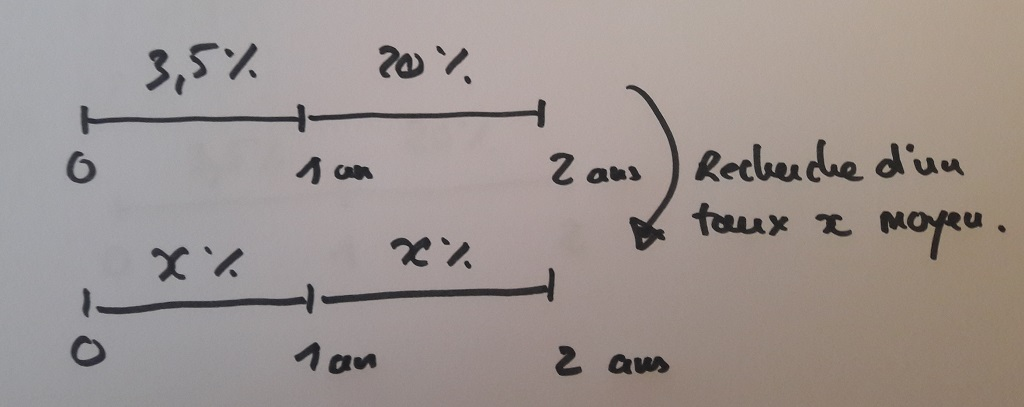
\includegraphics[width=8cm]{../Images/stat05}
    \end{figure} \\

    $C_1 = C_0 \times 1.035$ première année.
    \\ Puis deuxième année: $C_2 = C_1 \times 1.20 = C_0 \times 1.035 \times 1.2 = C_0 \times 1.242  $
    \\ \\
    Si on cherche maintenant le taux moyen $\bar{t} = 1 + x$ sur ces deux ans: \\
    $C_{11} = C_0 \times \bar{t}$ première année. \\
    Deuxième année : $C_{22} = C_{11} \times \bar{t} = C_0 \times \bar{t}^2 = C_0 \times 1.242 $ d'où :\\
    $\bar{t} = \sqrt{1.242} \simeq 1.114$ soit $x=0.114$, donc un taux moyen par an de : 11,4 \%.

    \subsection{généralisation}
    Soit une série statistique $(x_1,...x_n)$ de terme positifs, alors la moyenne géométrique de cette série est donnée par la formule suivante :
    \\
    $\bar{x} = ^n\sqrt{x_1 \times x_2 ... \times x_n}$ que l'on peut transformer en somme : $\bar{x} = \frac{1}{n}(\sum_{i=1}^n \log{x_i})$, ici la base du logarithme est quelconque.

    \end{document}